\documentclass{article}
\usepackage{amsmath}
\usepackage{float}
\usepackage{graphicx}
\usepackage[utf8]{inputenc}
\usepackage{listings}
  \lstset{captionpos=b, frame=single}
\newcommand{\colvec}[3]{
    \begin{pmatrix} #1 \\ #2 \\ #3 \end{pmatrix}
}

\begin{document}
  \title{MAT1110 - Obligatorisk oppgave 2.}
  \author{Robin A. T. Pedersen}
  \maketitle

  \section*{Oppg1. a)}
    Bilutleie i tre byer.

Første rad representerer by A sit tilskudd fra by A, B og C respektivt.
Tilsvarende for andre rad, by B, og tredje, by C.

$$A = \begin{pmatrix}
      0.4 & 0.3 & 0.3 \\
      0.3 & 0.5 & 0.2 \\
      0.3 & 0.2 & 0.5
      \end{pmatrix}$$

  \section*{Oppg1. b)}
    \paragraph{Egenverdi} \mbox{} \\
Vis at $\lambda$ er en egenverdi for A.
Da skal i såfall
$$det\begin{pmatrix}
     \lambda - 0.4 & -0.3 & -0.3 \\
     -0.3 & \lambda - 0.5 & -0.2 \\
     -0.3 & -0.2 & \lambda - 0.5
     \end{pmatrix} = 0$$

Vi regner ut og ser
$$\begin{vmatrix}
  \lambda - 0.4 & -0.3 & -0.3 \\
  -0.3 & \lambda - 0.5 & -0.2 \\
  -0.3 & -0.2 & \lambda - 0.5
  \end{vmatrix}$$
$$= \lambda - 0.4 \begin{vmatrix}
                  \lambda - 0.5 & -0.2 \\
                  -0.2 & \lambda - 0.5
                  \end{vmatrix}
    -(-0.3)\begin{vmatrix}
           -0.3 & -0.2 \\
           -0.3 & \lambda - 0.5
           \end{vmatrix}
    +(-0.3)\begin{vmatrix}
           -0.3 & \lambda - 0.5 \\
           -0.3 & - 0.2
           \end{vmatrix} $$
$$= \cdots = \lambda^3 - 1.4\lambda^2 + 0.43\lambda - 0.03$$

Hvis man velger $\lambda = 1$ får man
$$1 - 1.4 + 0.43 - 0.03 = 0$$

Altså er $\lambda = 1$ en egenverdi for $A$.



\paragraph{Egenvektor} \mbox{} \\
Før jeg starter må jeg vite hva $A\vec{v}$ er.
$$\begin{array}{c|c}
    & x \\
    & y \\
    & z \\
  \hline
    & 0.4x + 0.3y + 0.3z \\
  A & 0.3x + 0.5y + 0.2z \\
    & 0.3x + 0.2y + 0.5z
  \end{array}$$

For å finne egenvektoren
$$A\vec{v_1} = \lambda_1 \vec{v_1}$$
$$\implies \begin{pmatrix}
           -0.6 & 0.3 & 0.3 & 0 \\
           0.3 & -0.5 & 0.2 & 0 \\
           0.3 & 0.2 & -0.5 & 0
           \end{pmatrix}$$
$$\sim \cdots \sim \begin{pmatrix}
                1 & -\frac{5}{3} & \frac{2}{3} & 0 \\
                0 & 1 & -1 & 0 \\
                0 & 0 & 0 & 0
                \end{pmatrix}$$

Dette tilsier at
$$x = \frac{5}{3}y - \frac{2}{3}z$$
$$y = z$$
$$z = *$$

Hvis jeg velger $z = 1$ får man
$$\vec{v_1} = \begin{pmatrix}
              1 \\ 1 \\ 1
              \end{pmatrix}$$

  \section*{Oppg1. c)}
    \$ octave oppg1c.m
ans =

   0.10000
   0.30000
   1.00000

TODO

  \section*{Oppg1. d)}
    Ved nullte dag er antall biler i hver by
$$\vec{x_0} = \begin{pmatrix} 30 \\ 60 \\ 30 \end{pmatrix}$$



\paragraph{Lineærkombinasjon} \mbox{} \\
For å skrive $\vec{x_0}$ som en lineærkombinasjon av de tre egenvektorene
setter jeg opp følgende
$$\colvec{30}{60}{30}
  = u\colvec{1}{1}{1} + i\colvec{-2}{1}{1} + o\colvec{0}{-1}{1}$$
$$\colvec{30}{60}{30} = \colvec{u-2i}{u+i-o}{u+i+o}$$

Dette kan løses med radoperasjoner.
$$\begin{pmatrix}
  1 & -2 &  0 & 30 \\
  1 &  1 & -1 & 60 \\
  1 &  1 &  1 & 30
  \end{pmatrix}
  \sim \begin{pmatrix}
       1 & -2 &  0 & 30 \\
       0 &  3 & -1 & 30 \\
       0 &  3 &  1 & 0
       \end{pmatrix}
  \sim \begin{pmatrix}
       1 & -2 &  0   & 30 \\
       0 &  1 & -1/3 & 10 \\
       0 &  0 &  2   & -30
       \end{pmatrix}$$
Som gir $$u=40, \quad i=5, \quad o=-15$$
Altså er $$\vec{x_0} = 40\vec{v_1} + 5\vec{v_2} - 15\vec{v_3}$$



\paragraph{Etter n dager} \mbox{} \\
Antall biler i hver by etter n dager $\vec{x_n}$ er gitt ved
$$\vec{x_n} = A^n\vec{x_0}$$

Siden vi har $x_0$ som en lineærkombinasjon kan vi skrive
$$\vec{x_n} = A^n\vec{x_0}$$
$$= A^n(40\vec{v_1} + 5\vec{v_2} - 15\vec{v_3})$$
$$= 40A^n\vec{v_1} + 5A^n\vec{v_2} - 15A^n\vec{v_3}$$
$$= 40\lambda_1^n\vec{v_1} + 5\lambda_2^n\vec{v_2} - 15\lambda_3^n\vec{v_3}$$
$$= 40\vec{v_1} + 5(0.1)^n\vec{v_2} - 15(0.3)^n\vec{v_3}$$

Altså er
$$\vec{x_n} =
\colvec{40 - 10(0.1)^n}{40 + 5(0.1)^n + 15(0.3)^n}{40 + 5(0.1)^n - 15(0.3)^n}$$



\paragraph{Når n går mot uendelig} \mbox{} \\
Når n går mot uendelig vil de siste leddene ovenfor gå mot null.
Da står vi igjen med
$$\vec{x_\infty} = (40, 40, 40)$$

  \section*{Oppg1. e)}
    Plot antall biler i by A, B og C.

\begin{figure}[H]
  \centering
  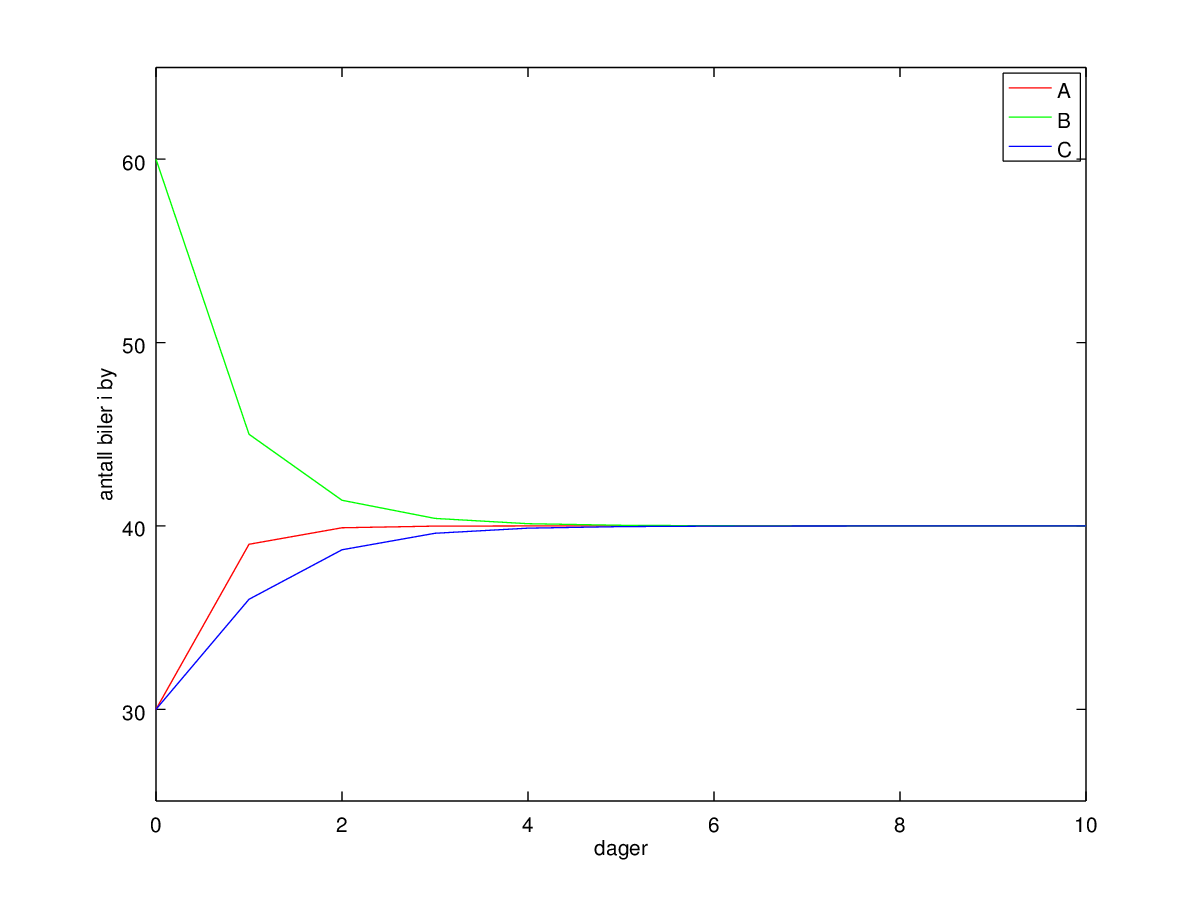
\includegraphics[width=\textwidth]{oppg1e}
  \caption{Fordeling av biler etter dager}
\end{figure}

\lstinputlisting[caption=Plottets tilhørende matlab kode]{oppg1e.m}


  \section*{Oppg2. a)}
    $$\vec{F}(x,y) = \begin{pmatrix} x^2y-y^2 \\ x-3 \end{pmatrix}$$
Finn nullpunktene til $\vec{F}$ ved regning.

$$\vec{F}(x,y) = \begin{pmatrix} 0 \\ 0 \end{pmatrix}$$
$$\implies \begin{matrix} x^2y-y^2=0 \\ x-3=0 \end{matrix}$$

Åpenbart må $x=3$. Da får vi
$$9y-y^2 = 0$$
Dette stemmer for $y=9$.
\\\\
Nullpunktet er altså $(3,9)$.

  \section*{Oppg2. b)}
    $$\vec{x_0} = (1,1)$$



\paragraph{Finn Jacobimatrisen til F} \mbox{} \\
$$J = \vec{F}'
    = \begin{pmatrix}
      \frac{\delta\vec{F_1}}{\delta x} & \frac{\delta\vec{F_1}}{\delta y} \\
      \frac{\delta\vec{F_2}}{\delta x} & \frac{\delta\vec{F_2}}{\delta y}
      \end{pmatrix}
    = \begin{pmatrix}
      2xy & x^2-2y \\
      1   & 0
      \end{pmatrix}$$



\paragraph{Første iterasjon med Newtons metode} \mbox{} \\
$$\vec{x_1} = \vec{x_0} - \vec{F}'(x_0)^{-1}\vec{F}(x_0)$$
$$ = (1,1) - \begin{pmatrix}2&-1\\1&0\end{pmatrix}^{-1} (0,-2) = \cdots$$

For å finne den inverse skjøter jeg på $I_2$ og radreduserer.
$$(\vec{F}(\vec{x_0}),I_2) =
  \begin{pmatrix} 2 & -1 & 1 & 0 \\ 1 & 0 & 0 & 1 \end{pmatrix}$$
$$\sim \begin{pmatrix} 1 & 0 & 0 & 1 \\ 0 & -1 & 1 & -2 \end{pmatrix}$$
$$\sim \begin{pmatrix} 1 & 0 & 0 & 1 \\ 0 & 1 & -1 & 2 \end{pmatrix}
  = (I_2, \vec{F}(\vec{x_0})^{-1})$$

Den inverse ganget med $\vec{F}(\vec{x_0})$.
$$\begin{array}{c c|c}
     &   &  0 \\
     &   & -2 \\
  \hline
   0 & 1 & -2 \\
  -1 & 2 & -4
  \end{array}$$

Fortsetter der jeg slapp
$$\vec{x_1} = \vec{x_0} - \vec{F}'(x_0)^{-1}\vec{F}(x_0)$$
$$ = (1,1) - \begin{pmatrix}2&-1\\1&0\end{pmatrix}^{-1} (0,-2)$$
$$ = (1,1) - (-2,-4) = (3,5)$$
Så $\vec{x_1} = (3,5)$



\paragraph{Andre iterasjon} \mbox{} \\
$$\vec{x_2} = \vec{x_1} - \vec{F}'(x_1)^{-1}\vec{F}(x_1)$$
$$= (3,5) - \begin{pmatrix}30&-1\\1&0\end{pmatrix}^{-1}(20,0)$$

Jeg inverterer det som inverteres må.
$$(\vec{F}'(x_1),I_2) = \begin{pmatrix}30&-1&1&0\\1&0&0&1\end{pmatrix}$$
$$\sim \begin{pmatrix}1&0&0&1\\0&-1&1&-30\end{pmatrix}$$
$$\sim \begin{pmatrix}1&0&0&1\\0&1&-1&30\end{pmatrix}
  = (I_2,\vec{F}'(x_1)^{-1})$$

Ganger det som ganges må.
$$\begin{array}{c c|c}
     &    &  20 \\
     &    &   0 \\
  \hline
   0 &  1 &   0 \\
  -1 & 30 & -20
  \end{array}$$

Fortsetter der jeg slapp
$$\vec{x_2} = \vec{x_1} - \vec{F}'(x_1)^{-1}\vec{F}(x_1)$$
$$= (3,5) - \begin{pmatrix}30&-1\\1&0\end{pmatrix}^{-1}(20,0)$$
$$= (3,5) - (0,-20) = (3,25)$$

Så er $\vec{x_2} = (3, 25)$

  \section*{Oppg2. c)}
    \paragraph{Newtons metode i matlab} \mbox{} \\
\lstinputlisting[caption=10 iterasjoner med matlab]{oppg2c.m}
\begin{lstlisting}[caption=Output]
$ octave oppg2c.m
x =

 Columns 1 through 8:

    1.0000    3.0000    3.0000    3.0000    3.0000    3.0000    3.0000    3.0000
    1.0000    5.0000   25.0000   15.2439   10.8143    9.2607    9.0071    9.0000

 Columns 9 and 10:

    3.0000    3.0000
    9.0000    9.0000
\end{lstlisting}

Den konvergerer det ene av nulltpunktene som jeg fant i oppgave 2a, (3,9).



\paragraph{Alternativt startpunkt} \mbox{} \\
Hva skjer hvis $x_0 = (1,0.1)$.

\begin{lstlisting}[caption=Output]
$ octave oppg2c-alt.m
x =

 Columns 1 through 8:

   1.00000   3.00000   3.00000   3.00000   3.00000   3.00000   3.00000   3.00000
   0.10000  -0.51250  -0.02620  -0.00008  -0.00000  -0.00000   0.00000   0.00000

 Columns 9 and 10:

   3.00000   3.00000
   0.00000   0.00000
\end{lstlisting}

Nå fant vi det andre nullpunktet fra 2a, $(3,0)$.

\end{document}
